\documentclass[ngerman,aspectratio=169]{beamer}
\usepackage[utf8]{luainputenc}
\usepackage[TS1,T1]{fontenc}
\usepackage{babel}
\usetheme[pagenum,navbar,ddc]{tud}
\usepackage{xcolor}
\usepackage{listings}
\usepackage{tikz}
\usepackage{multicol}

\newcommand{\theory}[1]{\text{Th(} #1 \text{)}}
\newcommand{\lang}[1]{\text{L(}#1{)}}

\title{TUN/TAP-Geräte\protect\\\mdseries Übersicht, Funktionsweise und Implementierung im Linux-Kernel\strut}
\subtitle{Proseminar Rechnernetze}
\author{Lucas Waclawczyk}

\newcommand*\inmm[1]{\pgfmathsetmacro\inmmwert{#1 / 1mm}\inmmwert}
\makeatletter
\newcommand*\inpt[1]{\setlength\@tempdima{#1}\the\@tempdima}
\makeatother

\AtBeginSection[]{\partpage{\usebeamertemplate***{part page}}}
\begin{document}
	\mode<presentation>{\setbeamertemplate{tud background}[image/shaded]{Seminarraum.jpg}{0.7}}
	\maketitle
	
	\mode<presentation>{\setbeamertemplate{page number in footline}[frame][text and total]}
	\frame{\frametitle{Inhalt}\tableofcontents}
	
	\section{Übersicht}
	\subsection{Rückblick Network Interfaces}
	\begin{frame}{Rückblick Network Interfaces}
		\begin{multicols}{2}
			\begin{itemize}
				\setlength{\itemsep}{1em}
				\item Interface = Schnittstelle
				\item muss nicht physisch sein\\(Virtual Network Interface)
			\end{itemize}
			\only<1>{
				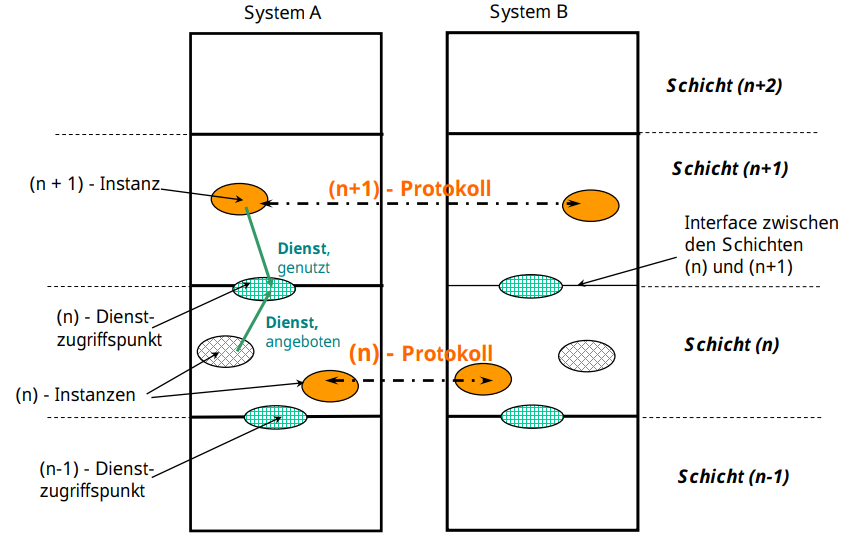
\includegraphics[width=\linewidth]{network_interface}
			}
			\only<2>{
				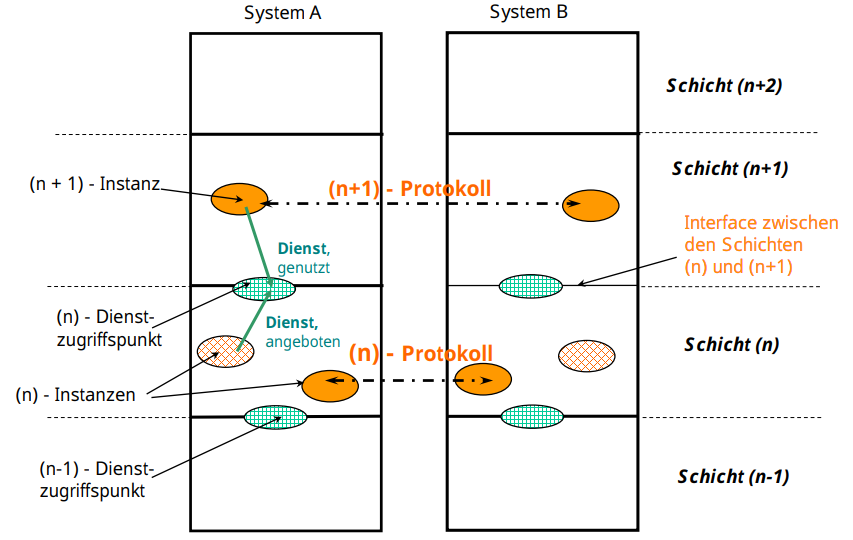
\includegraphics[width=\linewidth]{network_interface_colored}
			}
		\end{multicols}
	\end{frame}

	\subsection{Was sind TUN und TAP}
	\begin{frame}{Was sind TUN und TAP}
		\begin{itemize}
			\item Virtual Network Interfaces
			\item Linux
			\item \textit{OS $ \leftrightarrow $ Anwendung} statt \textit{physische Verbindung $ \leftrightarrow $ Hardware}
		\end{itemize}
	\end{frame}

	\subsection{Geschichte, Entstehung, Entwicklung}
	\begin{frame}{Geschichte, Entstehung, Entwicklung}
		höchstens drei Folien
	\end{frame}

	\section{Funktionsweise}
	\subsection{Set Up}
	\begin{frame}{Set Up}
		wahrscheinlich schematisch
	\end{frame}

	\subsection{Workflow}
	\begin{frame}{Workflow}
		wahrscheinlich schematisch		
	\end{frame}{Workflow}

	\subsection{Tear Down}
	\begin{frame}{Tear Down}
		wahrscheinlich schematisch
	\end{frame}

	\section{Implementierung}
	\subsection{Wo findet man das?}
	\begin{frame}{Wo findet man das?}
		Wo findet man Kernel Code, wo TUN / TAP Code, Erwähnung /dev/net/tun
	\end{frame}
	
	\subsection{Code}
	\begin{frame}{Code}
		etwa drei Folien
	\end{frame}

	\section{Quellen}
	\begin{frame}{Quellen}
		\begin{itemize}
			\item Skript und Übungsaufgaben der Vorlesung Rechnernetze, TU Dresden 2019 (präzise genug?)
			\item \url{https://backreference.org/2010/03/26/tuntap-interface-tutorial/}
			\item \url{https://www.elektronik-kompendium.de/sites/net/0811011.htm}
		\end{itemize}
	\end{frame}
\end{document}
